\section{Proof of Concept}
\label{app:poc}
A proof of concept (POC) was conducted to evaluate the extent to which the MAX4466 microphone can detect a change in distance or orientation of the emitted sound. 

\begin{figure}[ht!]
\begin{center}
    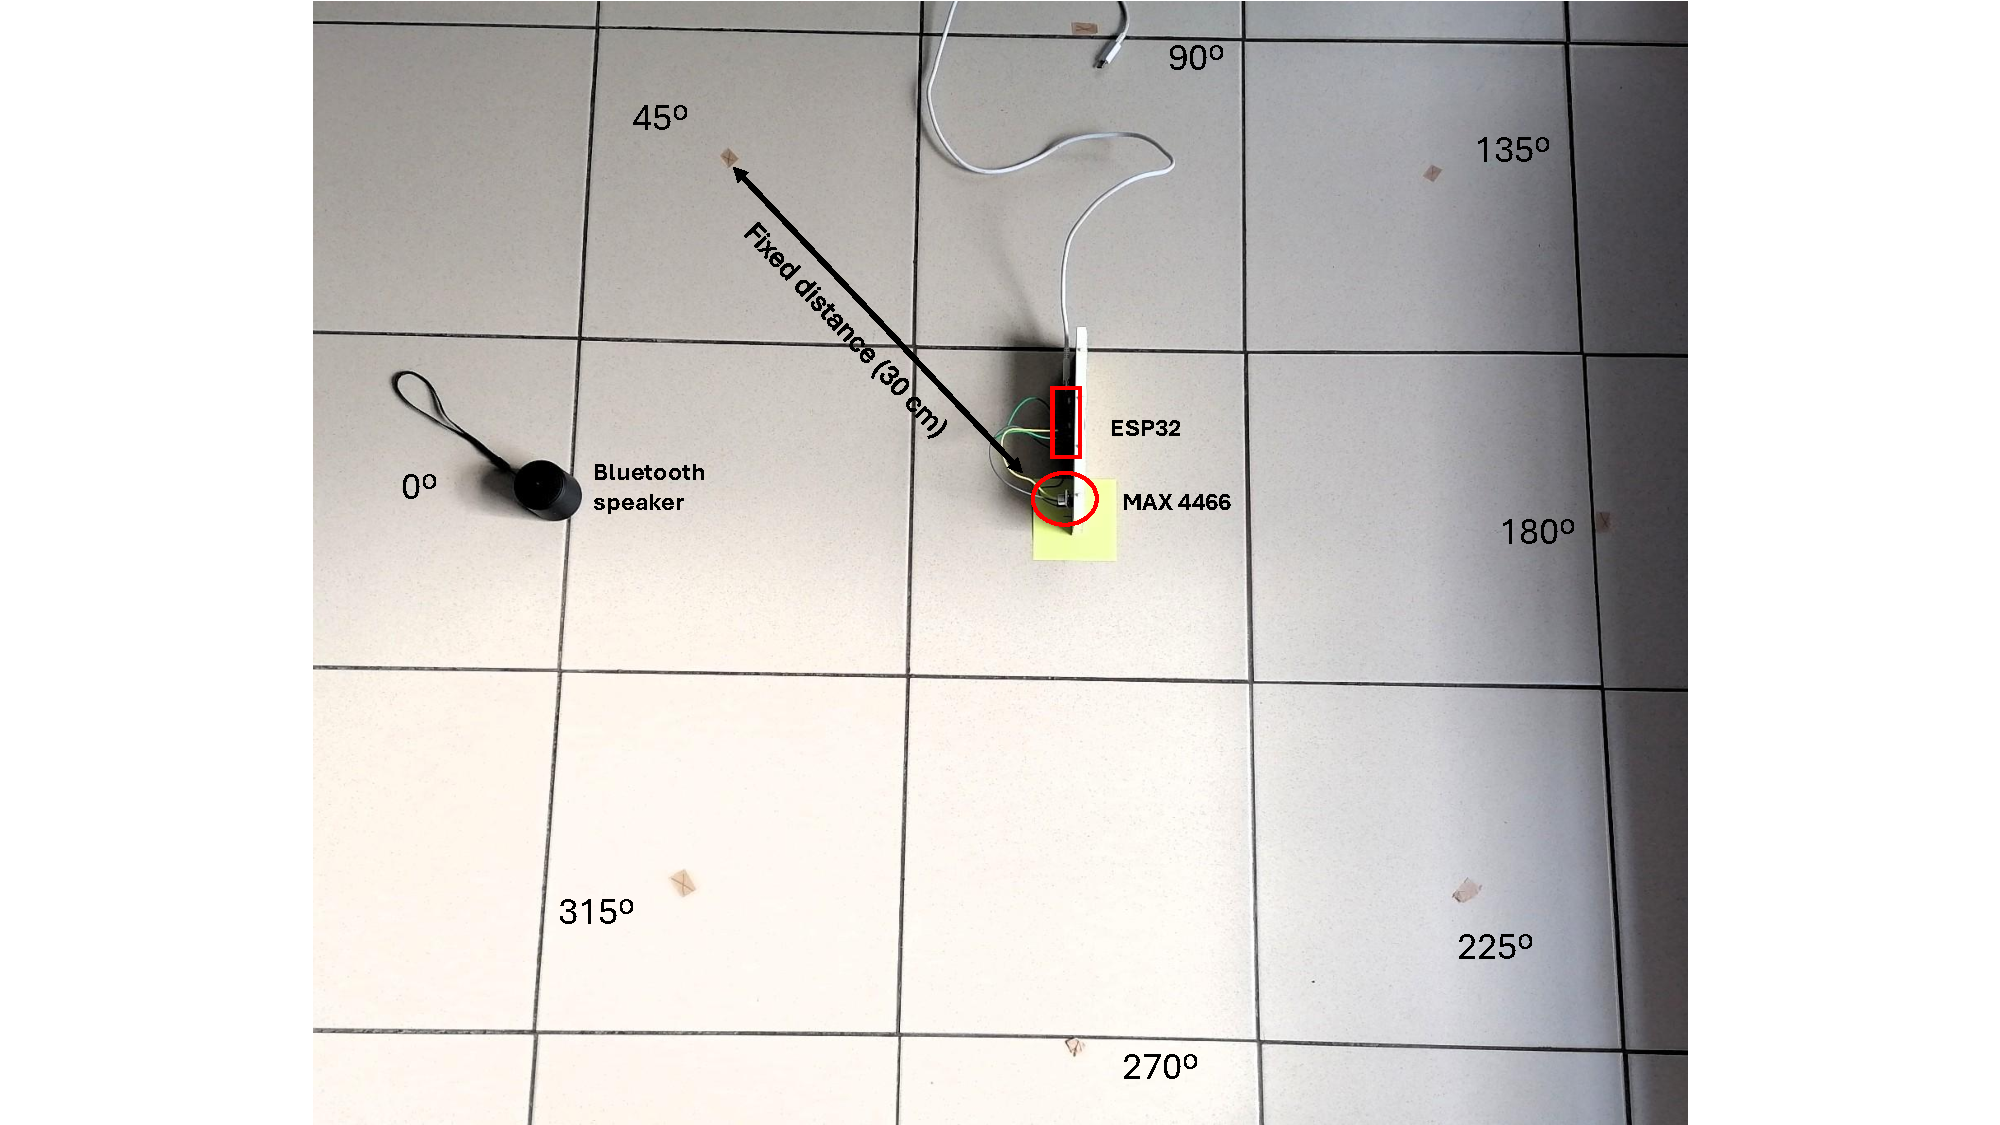
\includegraphics[width=0.7\linewidth]{poc.pdf}
    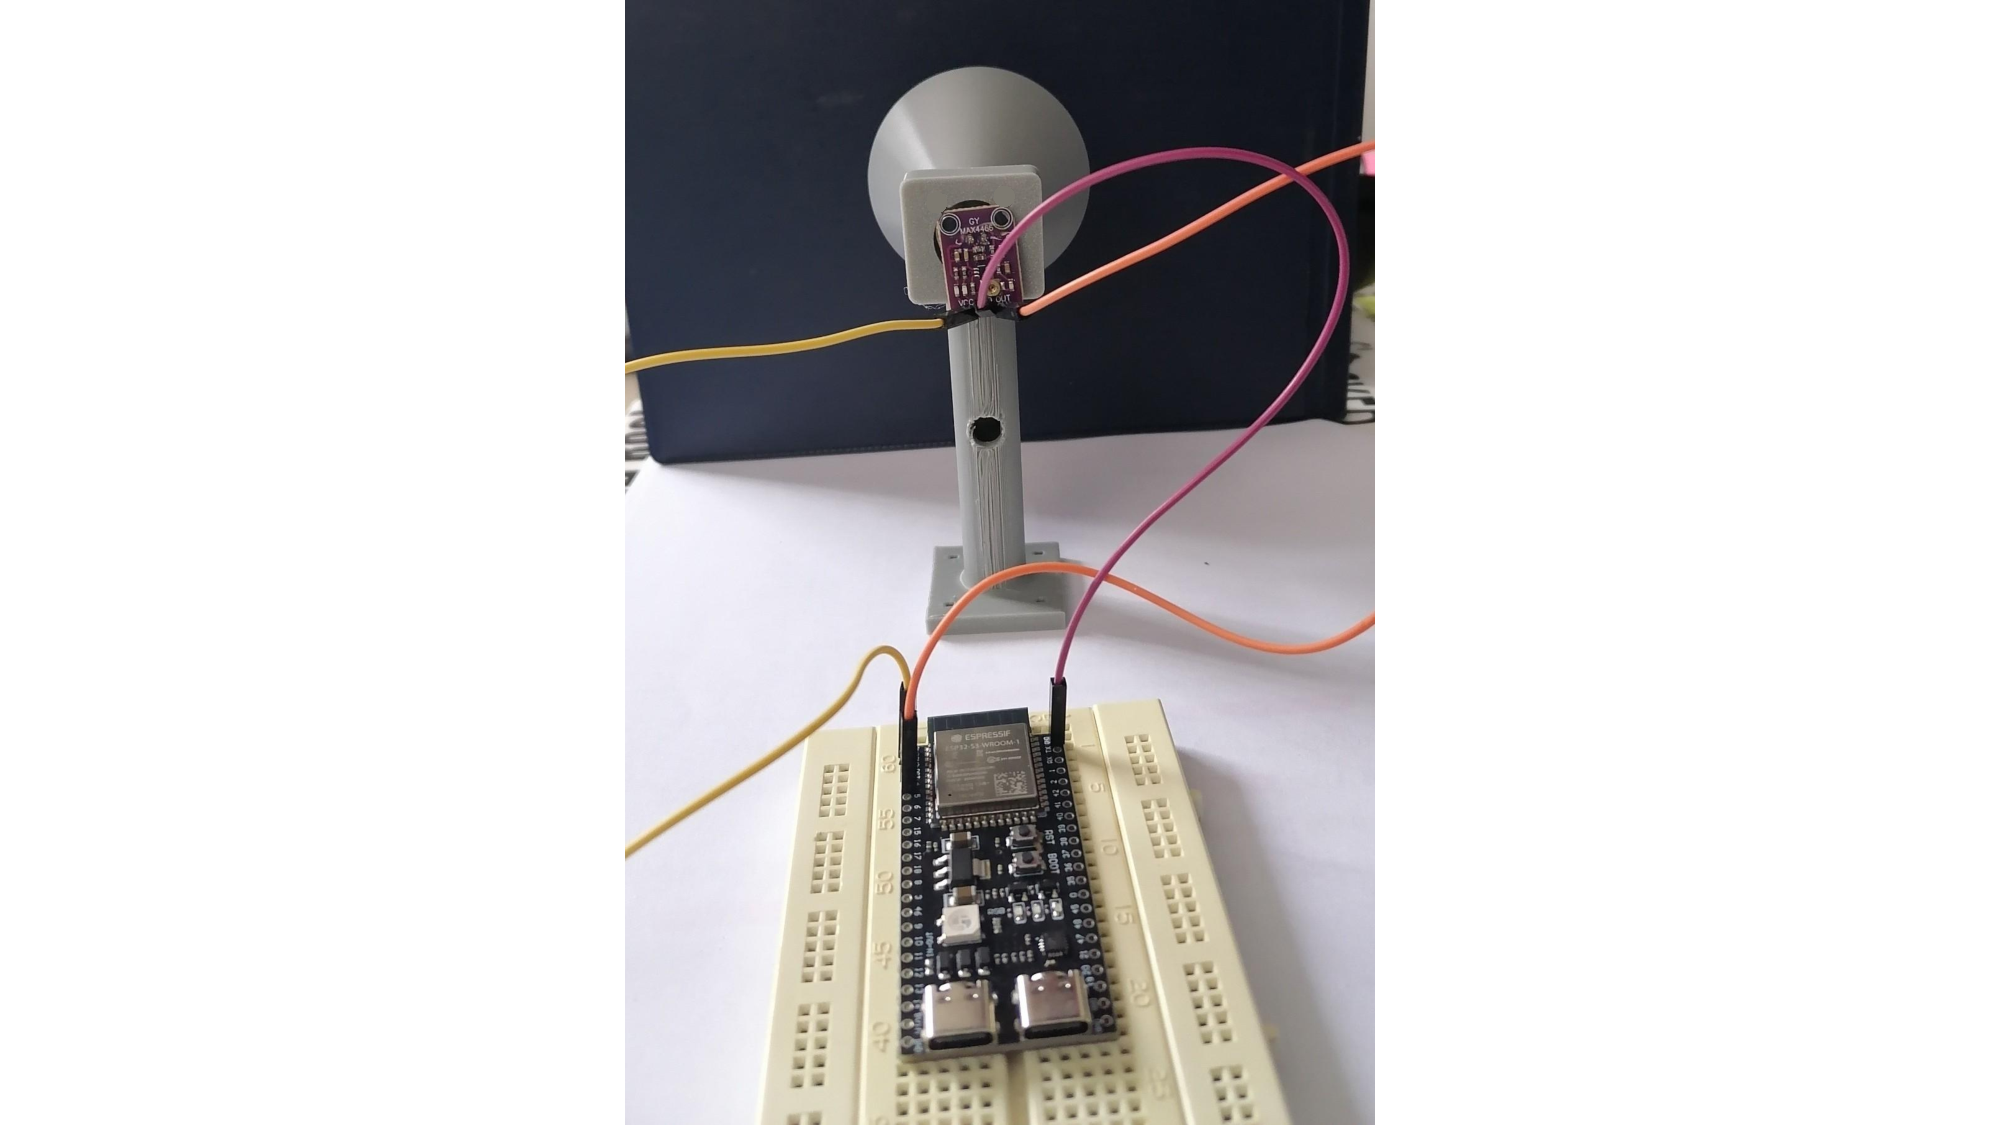
\includegraphics[width=0.2\linewidth]{mic_horn.pdf}
    \caption{Setup of the proof of concept including MAX 4466, ESP32, a breadboard, and a speaker with no horn (left) and zoom-in on the microphone + horn mounting for the second stage of the proof of concept (right).}
    \label{fig:poc}
\end{center}
\end{figure}

In the first stage, the microphone was connected to an ESP32 on a breadboard and placed at a fixed point, while a Bluetooth speaker was alternating across $8$ angular positions at a fixed distance of $30\text{ cm}$ (\autoref{fig:poc} left). The sound emitted consisted of a ``chirp'' at a constant frequency and regular intervals. Each angle sweep, at repeated measurements, exhibited peak-to-trough differences of approximately $5.2\text{--}7.8\text{ dB}$. The minimum amplitude was consistently recorded at $180^\circ$, while the maximum occurred near $0^\circ$ at around $63.0\text{ dB}$. Between $0^\circ$ and $180^\circ$, a drop of about $2\text{ dB}$ per $45^\circ$ was observed, with a symmetric behavior between $180^\circ$ and $360^\circ$ (\autoref{fig:polarplot} left). These results indicate the dependence of the response amplitude on the orientation of the sound source.

In the second stage, the same experiment was repeated with the 3D-printed directional horn attached to the microphone (\autoref{fig:poc} right). All other testing conditions were exactly the same. The results showed similar findings to the first stage of POC, but the signal level was approximately $2\text{ dB}$ higher in the horn pointing direction between $0^\circ\text{--}45^\circ$ and $315^\circ\text{--}360^\circ$, reaching approximately $65.0\text{ dB}$. This corresponds to a peak-to-trough difference of $10.3\text{--}10.5\text{ dB}$ (\autoref{fig:polarplot} right). This difference is higher than that recorded in the first stage, suggesting that the horn increases contrast of the measured signal between orientations. Therefore, these findings support the potential use of the horn in the assembly, although further testing at smaller angular increments is needed to achieve better sensitivity.

\begin{figure}[ht!]
\begin{center}
    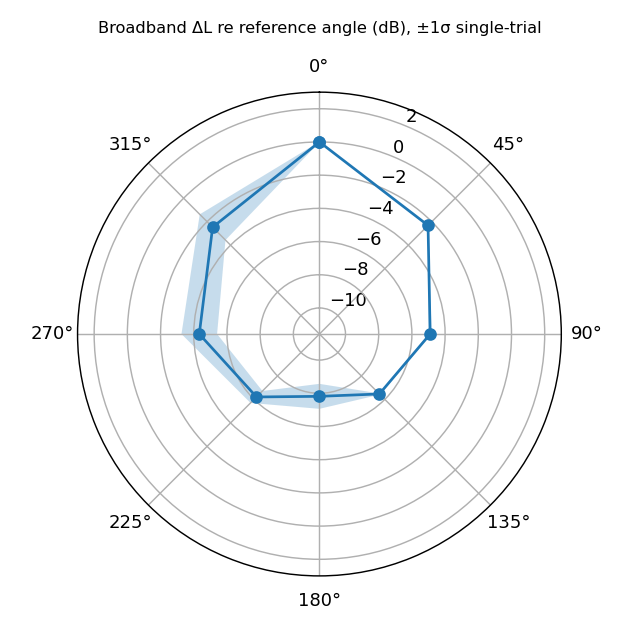
\includegraphics[width=0.43\linewidth]{bare1_summary_angle.png}
    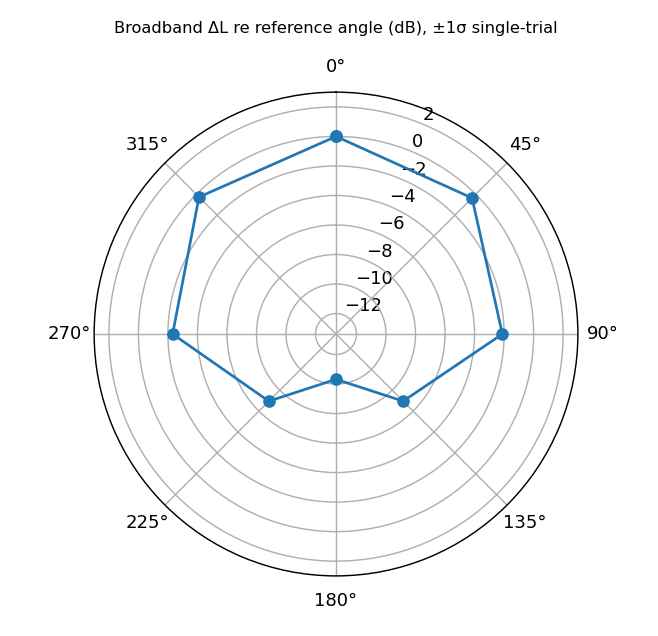
\includegraphics[width=0.43\linewidth]{horn1_summary_angle.png}
    \caption{\textbf{Measured directional gain profiles of the acoustic receiver setup.} Broadband relative sound level $\Delta L$ (dB) with respect to reference angle ($0^\circ$), evaluated across 8 angular increments ($45^\circ$ steps). \textbf{Left:} Baseline microphone setup without the directional horn. \textbf{Right:} Comparative profile with the 3D-printed directional horn.}
    \label{fig:polarplot}
\end{center}
\end{figure}

